\documentclass[11pt]{report}
\usepackage[utf8]{inputenc}
\usepackage[T1]{fontenc}
\usepackage[top=2.5cm, bottom=2.5cm, left=2cm, right=2cm]{geometry}
\usepackage{setspace}
\usepackage{graphicx}
\usepackage{float}
\usepackage{amsmath}
\usepackage{stmaryrd}
\usepackage{titlesec}
\usepackage{rotating}
\usepackage{alltt}
\usepackage{fancyvrb}
\usepackage{verbatimbox}
\usepackage{lipsum}
\usepackage{setspace}
\usepackage{tabto}
\usepackage{bussproofs}
\onehalfspacing
\titleformat{\chapter}[hang]{\bf\huge}{\thechapter}{2pc}{}

%-------------------------------------------------------
\let\oldabstract\abstract
\let\oldendabstract\endabstract
\makeatletter
\renewenvironment{abstract}
{\renewenvironment{quotation}%
               {\list{}{\addtolength{\leftmargin}{3em} % change this value to add or remove length to the the default
                        \listparindent 1.5em%
                        \itemindent    \listparindent%
                        \rightmargin   \leftmargin%
                        \parsep        \z@ \@plus\p@}%
                \item\relax}%
               {\endlist}%
\oldabstract}
{\oldendabstract}
\makeatother

\makeatletter
\newcommand{\verbatimfont}[1]{\renewcommand{\verbatim@font}{\normalfont#1}}
\makeatother

\begin{document}
\begin{center}

\includegraphics[scale = 1]{index.png}
\end{center}

\pagestyle{empty}
\vspace*{\stretch{8}}


\centerline{\textbf{\Huge Parser Documentation}}
\bigbreak\bigbreak
\bigbreak\bigbreak

\centerline{ {\Large Estelle Alauzy}}
\vspace*{\stretch{1}}
\centerline{ {\Large  Chervin Amirkaveh}}


 \vfill
 \vspace*{\stretch{10}}
\centerline{\large June 2019}
\vspace*{\stretch{1}}






%%%%%%%%%%%%%%%%%%%%%%%%%%%%%%%%%%%%%%%%%%%%%%%%%%%%%%%%%%%%%%%%%%%%%%%%%%%%
%%%%%%%%%%%%%%%%%%%%%%%%%%%%%%%%%%%%%%%%%%%%%%%%%%%%%%%%%%%%%%%%%%%%%%%%%%%%

\newpage
\centerline{\textbf{\Huge Context}}
\vspace*{3pt}
\vspace*{20pt}

\tabto{1cm}Concurrency has become increasingly important in the last several years, increasing the need for verification tools for concurrent programs for languages such as Go, Erlang, and more. Although concurrent program equivalence has been studied for decades in the context of process algebras, a significant amount of theoretical results in this area have not reached the practice of software verification. 
\\ \\
\tabto{1cm}For example, one of the most well-established modelling language for concurrent, communicating systems is the pi-calculus. Researchers have used this language to develop some of the
most powerful techniques for program equivalence in a concurrent setting, which are based on (weak) bisimulation and its extensions (environmental bisimulation, up-to-context technique, up-to-* technique). However there is a distinct absence of tools for verifying the equivalence of pi-calculus terms.
\\ \\
\tabto{1cm}It is in this context that we have started the project to create a language that could be use as an intermediate language for a tool using a “bisimulation engine” back-end to prove the equivalence of programs.

\newpage
\centerline{\textbf{\Huge Description of the language}}
\vspace*{3pt}
\vspace*{20pt}
\tabto{1cm}First of all, this language is procedural meaning that procedures/functions are declared at top-level and can then be called anywhere in the program. This language contains basic and convenient features that you can find in most programming languages : basic types (integer, boolean, char, string), lists, 
tuples, local and global variables, functions declaration and call, different binary and unary operators for expressions, if-then-else, while and return instructions, ...
\\ \\
\tabto{1cm}However, what is making this language different from others is the integration of pi-calculus notions inside the language. Indeed, it is possible to declare channels as variables. Those channels can be used in different instructions : newChan, send and receive.
\begin{itemize}
\item \ ch = newChan(): create a new channel of the same type as the variable ch and assign it this new channel to it.
\item \ send(ch,e): send the expression e along the channel ch
\item \ v = receive(ch): receive an expression along the channel ch and assign it to the variable v
\end{itemize}

\tabto{1cm}The notion of input-guarded choice is also available in this language thanks to the instruction choose. The choose instructions allows you to use prefixes (new, send, receive, spawn, tau). The purpose of this instruction is the following: when the action of the prefix is possible, the action is made and the instructions corresponding to that prefix are executed after. In the case where actions of two different prefixes are possible at the same time, the program will choose one of them in a non-deterministic way.
\\ \\
\tabto{1cm} Finally, we have also added the instruction spawn to represent the parallelization of processes. Spawn can be seen as the "|" operator of the pi-calculus. It is important to note that spawn is not representing the immediate launch of a new thread. Indeed, when you code a sequence of spawn instructions, it's represents a simultaneous launch of all processes and not a sequential launch. The function and expression passed in arguments of the spawn instruction are used to create the new process.
\\ \\
\tabto{1cm} You will find below the grammar describing the language and a section about technical decisions that have impacted the language.

\newpage
\centerline{\textbf{\Huge Grammar : Backus-Naur form (BNF)}}
\vspace*{20 pt}
\vspace*{3pt}
\begin{Verbatim}[fontfamily=textsf]
Program ::= TypeDecla Program
            | FuncDecla Program
            | VariableDecla Program
            | FuncDecla CallMain
            | VariableDecla CallMain
\end{Verbatim}
\vspace*{3pt}

\begin{verbnobox}[\normalfont]
FuncDecla ::= func FuncType name (Parameters) Body
\end{verbnobox}
\vspace*{3pt}

\begin{verbnobox}[\normalfont]
TypeDecla ::= type name = Typ
\end{verbnobox}
\vspace*{3pt}

\begin{verbnobox}[\normalfont]
Parameters ::= Typ identifier | Typ identifier , Parameters
\end{verbnobox}
\vspace*{3pt}

\begin{verbnobox}[\normalfont]
Body ::= { Instruction } | { def VariableDeclas in Instruction }
\end{verbnobox}
\vspace*{3pt}

\begin{verbnobox}[\normalfont]
VariableDecla ::= Typ identifier | Typ ( TupleDecla )
\end{verbnobox}
\vspace*{3pt}

\begin{verbnobox}[\normalfont]
TupleDecla ::= identifier | identifier , TupleDecla
\end{verbnobox}
\vspace*{3pt}

\begin{verbnobox}[\normalfont]
VariableDeclas ::= VariableDecla 
                    | VariableDeclas ; 
                    | VariableDecla ; VariableDeclas
\end{verbnobox}
\vspace*{3pt}

\begin{verbnobox}[\normalfont]
Instruction ::= ; Instruction
               |
               | Bintruction 
               | Binstruction ; Instruction
\end{verbnobox}
\vspace*{3pt}

\begin{verbnobox}[\normalfont]
Binstruction ::= Expression = Expression 
                 | Expression = name ( ExpressionSeq )
                 | name ( ExpressionSeq )
                 | Expression = receive ( identifier )
                 | send ( identifier , Expression )
                 | if ( Expression ) { Instruction } else { Instruction }
                 | while ( Expression ) { Instruction }
                 | choose { Choices }
                 | spawn name ( ExpressionSeq )
                 | Expression = newChan()
                 | return
                 | return Expression
                 | return name (ExpressionSeq)
\end{verbnobox}
\vspace*{3pt}

\begin{verbnobox}[\normalfont]
Choices ::= Prefix -> { Instruction } Choices | Prefix -> { Instruction }
\end{verbnobox}
\vspace*{3pt}

\begin{verbnobox}[\normalfont]
Prefix ::= | tau
         | | send ( identifier , Expression )
         | | Expression = receive ( identifier )
         | | Expression = newChan()
         | | spawn name ( ExpressionSeq )
\end{verbnobox}
\vspace*{3pt}

\begin{verbnobox}[\normalfont]
Expression ::= - Expression
               | head ( Expression )
               | tail ( Expression )
               | odd ( Expression )
               | even ( Expression )
               | Expression + Expression
               | Expression - Expression
               | Expression || Expression
               | Expression * Expression
               | Expression / Expression
               | Expression && Expression
               | Expression == Expression
               | Expression != Expression 
               | Expression < Expression
               | Expression > Expression
               | if ( Expression ) { Expression } else { Expression }
               | ( ExpressionSeq )
               | Value
               | identifier
\end{verbnobox}
\vspace*{3pt}

\begin{verbnobox}[\normalfont]
ExpressionSeq ::= Expression | Expression , ExpressionSeq
\end{verbnobox}
\vspace*{3pt}

\begin{verbnobox}[\normalfont]
Constant ::= integer
             | ' char '
             | " string "
             | true
             | false
\end{verbnobox}
\vspace*{3pt}

\begin{verbnobox}[\normalfont]
Value ::= Constant | { ValueSeq }
\end{verbnobox}
\vspace*{3pt}

\begin{verbnobox}[\normalfont]
ValueSeq ::= Value | Value , ValueSeq
\end{verbnobox}
\vspace*{3pt}

\begin{verbnobox}[\normalfont]
Typ ::= int
      | boolean
      | string
      | char
      | channel Typ
      | list [ Types ]
      | ( Types )
      | identifier
\end{verbnobox}
\vspace*{3pt}

\begin{verbnobox}[\normalfont]
Types ::= Typ | Typ , Types
\end{verbnobox}
\vspace*{3pt}

\begin{verbnobox}[\normalfont]
FuncType ::= void | Typ
\end{verbnobox}
\vspace*{3pt}

\begin{verbnobox}[\normalfont]
CallMain ::= start name ( ExpressionSeq )
\end{verbnobox}
\vspace*{3pt}

\newpage
\centerline{\textbf{\Huge Technical choices}}
\vspace*{3pt}
\vspace*{10pt}
\tabto{0cm} {\Large \textbf{Conflicts resolution}}
\\ \\ 
\tabto{1cm} In order to remove ambiguities in our grammar and so resolve shift/reduce conflicts we have added some rules. It is important to note that in our grammar the majority of our conflicts refer to binary operators.  \\ \\ \\
By declaring precedence and associative rules for all tokens involved in the conflicts, this force derivations to be done in a particular way.
\\ \\ 
\tabto{2cm} \textbf{Associativity}
\\ \\
\tabto{1cm} The first way to make unambiguous our grammar is by establishing associative rules for an operator "op". Theses rules determines how to interpret the operator's repetition: if "x op y op z" must be considered as "(x op y) op z" or "x op (y op z)". \\ \\
There are three different ways to specify them. 
\begin{itemize}
\item \%right:  makes the operator right-associative
\item \%left: makes the operator left-associative
\item \%nonassoc: makes the association incorrect, i.e.: "x op y op z" will be considered as a syntax error.
\end{itemize}
We have decided that the operators: $*$, $+$, $-$, $/$, $=$, $\ne$, $\&\&$ and $||$ are left-associative and that for the operators $>$ and $<$ the association is incorrect.
\\ \\ \\
\tabto{2cm} \textbf{Precedence}
\\ \\
\tabto{1cm} The second way to make unambiguous our grammar is by imposing the precedence of one operator over the other. The relative precedence between the different operators is defined by the order in which they are declared. The first declared has the lowest precedence and so the last declared has the highest precedence. We have chosen the order of the precedence in way that the different operators respect the arithmetic logic.
\\ \\
\newpage
We have also used semi-colons to resolve conflicts. \\ \\
\tabto{2cm} \textbf{Semi-colon} \\ \\
\tabto{1cm}Semi-colons allow to separate instructions from each other and so that avoid shift-reduce conflicts at the level of the assign and return operators. It also makes our grammar more resistant and so easier for someone to add new instructions without causing conflicts. \\ \\
\tabto{1cm} In our grammar, the semicolon should not be interpreted as an end of line indication but simply as a separator between variable declarations or instructions:
\begin{itemize}
\item For instructions: a semicolon sequence is translated by the parser as a sequence of empty instructions.
\item For variable declarations: this is not possible, however it is possible to end the declarations with a semicolon without causing an error syntax but it makes no sense in our grammar. We have implemented this to avoid mistakes due to the use of other languages.
\end{itemize}

\tabto{0cm} {\Large \textbf{Title}}



\newpage
\centerline{\textbf{\Huge Type rules}}
\vspace*{3pt}
\vspace*{20pt}


\tabto{0cm} {\large \textbf{Binary Operator}}
\begin{prooftree}
\AxiomC{$\Gamma_t ; \ \Gamma_v ; \vdash e_1: T_1 $}
\AxiomC{$\Gamma_t ; \ \Gamma_v \vdash e_2 : T_2$}
\AxiomC{$T_1 \times T_2 \in dom$ op}
\AxiomC{$T \in codom$ op}
\QuaternaryInfC{$\Gamma_t ; \ \Gamma_v ; \vdash e_1 \ op \ e_2 : T $}
\end{prooftree}

\tabto{0cm} {\large \textbf{Unary Operator}}
\begin{prooftree}
\AxiomC{$\Gamma_t ; \ \Gamma_v \vdash e : T $}
\AxiomC{$T \in dom$ op}
\AxiomC{$T' \in codom$ op}
\TrinaryInfC{$\Gamma_t ; \ \Gamma_v \vdash op \ e : T' $}
\end{prooftree}

\tabto{0cm} {\large \textbf{Negate Operator}}
\begin{prooftree}
\AxiomC{$\Gamma_t ; \ \Gamma_v \vdash e : T $}
\AxiomC{$T \in dom \ -$}
\AxiomC{$T' \in codom \ -$}
\TrinaryInfC{$\Gamma_t ; \ \Gamma_v \vdash - \ e : T' $}
\end{prooftree}

\tabto{0cm} {\large \textbf{Condition}}
\begin{prooftree}
\AxiomC{$\Gamma_t ; \ \Gamma_v \vdash e_1 : bool $}
\AxiomC{$\Gamma_t ; \ \ \Gamma_v \vdash e_2 : T $}
\AxiomC{$\Gamma_t ; \ \Gamma_v \vdash e_3 : T $}
\TrinaryInfC{$\Gamma_t ; \ \Gamma_v \vdash if \ e_1 \ then \ e_2 \ else \ e_3 : T $}
\end{prooftree}

\tabto{0cm} {\large \textbf{Tuple}}
\begin{prooftree}
\AxiomC{$\Gamma_t ; \ \Gamma_v \vdash e_1 : T_1$}
\AxiomC{$\Gamma_t ; \ \Gamma_v \vdash e_2 : T_2 $}
\AxiomC{$\ldots$}
\AxiomC{$\Gamma_t ; \ \Gamma_v \vdash e_n : T_n $}
\QuaternaryInfC{$\Gamma_t ; \ \Gamma_v \vdash (e_1,e_2,\ldots,e_n) : T_1 \times T_2 \times \ldots \times T_n)$}
\end{prooftree}

\tabto{0cm} {\large \textbf{List of Values}}
\begin{prooftree}
\AxiomC{$\Gamma_t ; \ \Gamma_v \vdash e_1 : T$}
\AxiomC{$\Gamma_t ; \ \Gamma_v \vdash e_2 : T $}
\AxiomC{$\ldots$}
\AxiomC{$\Gamma_t ; \ \Gamma_v \vdash e_n : T $}
\QuaternaryInfC{$\Gamma_t ; \ \Gamma_v \vdash [e_1,e_2,\ldots,e_n] : list [T]$}
\end{prooftree}

\tabto{0cm} {\large \textbf{Identifier}}
\begin{prooftree}
\AxiomC{$ x : T \in \Gamma_v$}
\UnaryInfC{$\Gamma_t ; \ \Gamma_v \vdash x : T$}
\end{prooftree}

\tabto{0cm} {\large \textbf{Assignment}}
\begin{prooftree}
\AxiomC{$\Gamma_t ; \ \Gamma_v ; \vdash a : T_a $}
\AxiomC{$\Gamma_t ; \ \Gamma_v \vdash e : T_e$}
\AxiomC{$ T_a = T_e $}
\TrinaryInfC{$\Gamma_t ; \ \Gamma_v ; \vdash a = e : void $}
\end{prooftree}

\tabto{0cm} {\large \textbf{Function Call with return}}
\begin{prooftree}
\AxiomC{$\Gamma_t ; \ \Gamma_v \vdash e_1 : T_2 $}
\AxiomC{$\Gamma_t ; \ \Gamma_v \vdash e_2 : T_1 \rightarrow T_2 $}
\AxiomC{$\Gamma_t ; \ \Gamma_v \vdash e_3 : T_1 $}
\TrinaryInfC{$\Gamma_t ; \ \Gamma_v \vdash e_1 = e_2 (e_3) : T_2 $}
\end{prooftree}

\tabto{0cm} {\large \textbf{Function Call without return}}
\begin{prooftree}
\AxiomC{$\Gamma_t ; \ \Gamma_v \vdash e_1 : T_1 \rightarrow void$}
\AxiomC{$\Gamma_t ; \ \Gamma_v \vdash e_2 : T_1 $}
\BinaryInfC{$\Gamma_t ; \ \Gamma_v \vdash e_1(e_2) : void $}
\end{prooftree}

\newpage

\tabto{0cm} {\large \textbf{While}}
\begin{prooftree}
\AxiomC{$\Gamma_t ; \ \Gamma_v \vdash e_1 : bool$}
\AxiomC{$\Gamma_t ; \ \Gamma_v \vdash e_2 : T $}
\BinaryInfC{$\Gamma_t ; \ \Gamma_v \vdash while(e_1) \ \{ e_2 \} : T $}
\end{prooftree}

\tabto{0cm} {\large \textbf{Return void}}
\begin{prooftree}
\AxiomC{$ $}
\UnaryInfC{$\Gamma_t ; \ \Gamma_v \vdash return : void $}
\end{prooftree}

\tabto{0cm} {\large \textbf{Return Expression }}
\begin{prooftree}
\AxiomC{$\Gamma_t ; \ \Gamma_v \vdash e : T$}
\UnaryInfC{$\Gamma_t ; \ \Gamma_v \vdash return \ e : T $}
\end{prooftree}

\tabto{0cm} {\large \textbf{Send Instruction}}
\begin{prooftree}
\AxiomC{$\Gamma_t ; \ \Gamma_v \vdash T $}
\AxiomC{$\Gamma_t ; \ \Gamma_v \vdash c : chan \ T $}
\AxiomC{$\Gamma_t ; \ \Gamma_v \vdash e : T $}
\TrinaryInfC{$\Gamma_t ; \ \Gamma_v \vdash send(c,e) : void $}
\end{prooftree}

\tabto{0cm} {\large \textbf{Receive Instruction}}
\begin{prooftree}
\AxiomC{$\Gamma_t ; \ \Gamma_v \vdash T $}
\AxiomC{$\Gamma_t ; \ \Gamma_v \vdash c : chan \ T $}
\AxiomC{$\Gamma_t ; \ \Gamma_v \vdash a : T $}
\TrinaryInfC{$\Gamma_t ; \ \Gamma_v \vdash a = receive(c) : void $}
\end{prooftree}

\tabto{0cm} {\large \textbf{Spawn Instruction}}
\begin{prooftree}
\AxiomC{$\Gamma_t ; \ \Gamma_v \vdash e_1 : T_1 \rightarrow void$}
\AxiomC{$\Gamma_t ; \ \Gamma_v \vdash e_2 : T_1 $}
\BinaryInfC{$\Gamma_t ; \ \Gamma_v \vdash spawn \ e_1(e_2) : void $}
\end{prooftree}

\tabto{0cm} {\large \textbf{NewChan Instruction}}
\begin{prooftree}
\AxiomC{$\Gamma_t ; \ \Gamma_v \vdash T $}
\AxiomC{$\Gamma_t ; \ \Gamma_v \vdash a : chan \ T $}
\BinaryInfC{$\Gamma_t ; \ \Gamma_v \vdash a = newChan() : void $}
\end{prooftree}

\tabto{0cm} {\large \textbf{Choose Instruction}}
\begin{prooftree}
\AxiomC{$\Gamma_t ; \ \Gamma_v \vdash p_1 : void \ \ldots \ \Gamma_t ; \ \Gamma_v \vdash p_n : void $}
\AxiomC{$\Gamma_t ; \ \Gamma_v \vdash i_1 : T \ \ldots \ \Gamma_t ; \ \Gamma_v \vdash i_n : T $}
\BinaryInfC{$\Gamma_t ; \ \Gamma_v \vdash Choose \{ \ \ | \ p_1 -> i_1 \ \ | \ \ldots \ | \ p_n -> i_n \ \ \} : T $}
\end{prooftree}

\tabto{0cm} {\large \textbf{Sequence of Instructions}}
\begin{prooftree}
\AxiomC{$\Gamma_t ; \ \Gamma_v \vdash e_1 : void$}
\AxiomC{$\Gamma_t ; \ \Gamma_v \vdash e_2 : T $}
\BinaryInfC{$\Gamma_t ; \ \Gamma_v \vdash e_1 \ ; \ e_2 : T $}
\end{prooftree}

\newpage

\tabto{0cm} {\large \textbf{Variable Declaration}}
\begin{prooftree}
\AxiomC{$\Gamma_t ; \ \Gamma_v \vdash T $}
\UnaryInfC{$\Gamma_t ; \ \Gamma_v \vdash T \ x $}
\end{prooftree}

\tabto{0cm} {\large \textbf{Function Declaration}}
\begin{prooftree}
\AxiomC{$\Gamma_t ; \ \Gamma_v \vdash T $}
\AxiomC{$\Gamma^\prime := \Gamma_t ; \ \Gamma_v ; \ x_1 : T_1 ; \ \ldots \ x_n : T_n  $}
\AxiomC{$\Gamma^\prime \vdash \overrightarrow{declaVar} $}
\AxiomC{$\Gamma^\prime ; \ \overrightarrow{declaVar} \vdash i : T $}
\QuaternaryInfC{$\Gamma_t ; \ \Gamma_v \vdash func \ T \ name \ (T_1 \ x_1 , \ \ldots , \ T_n \ x_n) \ \{ \ def \ \overrightarrow{declaVar} \ in \ i \}$}
\end{prooftree}

\newpage
\centerline{\textbf{\Huge Examples}}
\vspace*{3pt}
\vspace*{20pt}
Communicating and mobile systems : the $\pi$-calculus - Robin Milner : The mobile phones system

\begin{center}
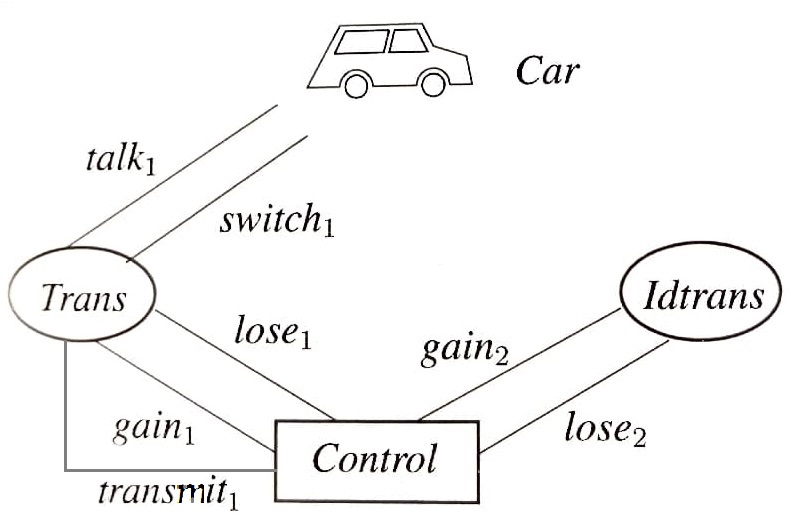
\includegraphics[scale = 0.5]{mobile-phone-system.jpg}
\end{center}
Add the Description of the example from the book p-82

To allow the control to know when it needs to act we add an other channel between Control and Trans named transmit1. This channel transmit the message received by Trans since Car. This message is an integer which represents the position of the car. We arbitrarily decide the position when links between the Trans and the car must be switch to the other trans : Idtrans. So, when the position is greater than the threshold the Control tells to Trans to lose the car and to IdTrans to gain the car.

\end{document}
